\documentclass{ximera}
%% You can put user macros here
%% However, you cannot make new environments

\listfiles

\graphicspath{{./}{firstExample/}{secondExample/}}

\usepackage{tikz}
\usepackage{tkz-euclide}
\usepackage{tikz-3dplot}
\usepackage{tikz-cd}
\usetikzlibrary{shapes.geometric}
\usetikzlibrary{arrows}
\usetkzobj{all}
\pgfplotsset{compat=1.13} % prevents compile error.

%\renewcommand{\vec}[1]{\mathbf{#1}}
\renewcommand{\vec}{\mathbf}
\newcommand{\RR}{\mathbb{R}}
\newcommand{\dfn}{\textit}
\newcommand{\dotp}{\cdot}
\newcommand{\id}{\text{id}}
\newcommand\norm[1]{\left\lVert#1\right\rVert}
 
\newtheorem{general}{Generalization}
\newtheorem{initprob}{Exploration Problem}

\tikzstyle geometryDiagrams=[ultra thick,color=blue!50!black]

%\DefineVerbatimEnvironment{octave}{Verbatim}{numbers=left,frame=lines,label=Octave,labelposition=topline}



\usepackage{mathtools}


\title{Where was Eye? (part 2)} \license{CC BY-NC-SA 4.0}

\begin{document}

\begin{abstract}
We determine the location of the camera based on a photograph it took.
\end{abstract}
\maketitle

\section*{Where was Eye? (part 2)}


In this part of the activity, you will take your own photos from a known height to test the formula you had developed in Part 1.  

\subsubsection*{Directions}
In groups of two or three, you will use a phone to take photos of a long desk, a sheet of paper or a hallway while holding your phone at a known height.

\begin{itemize}
    \item Make sure that the camera is located in the center of the hallway/desk/paper so that the triangle formed by the edges is isosceles.
    \begin{image}
         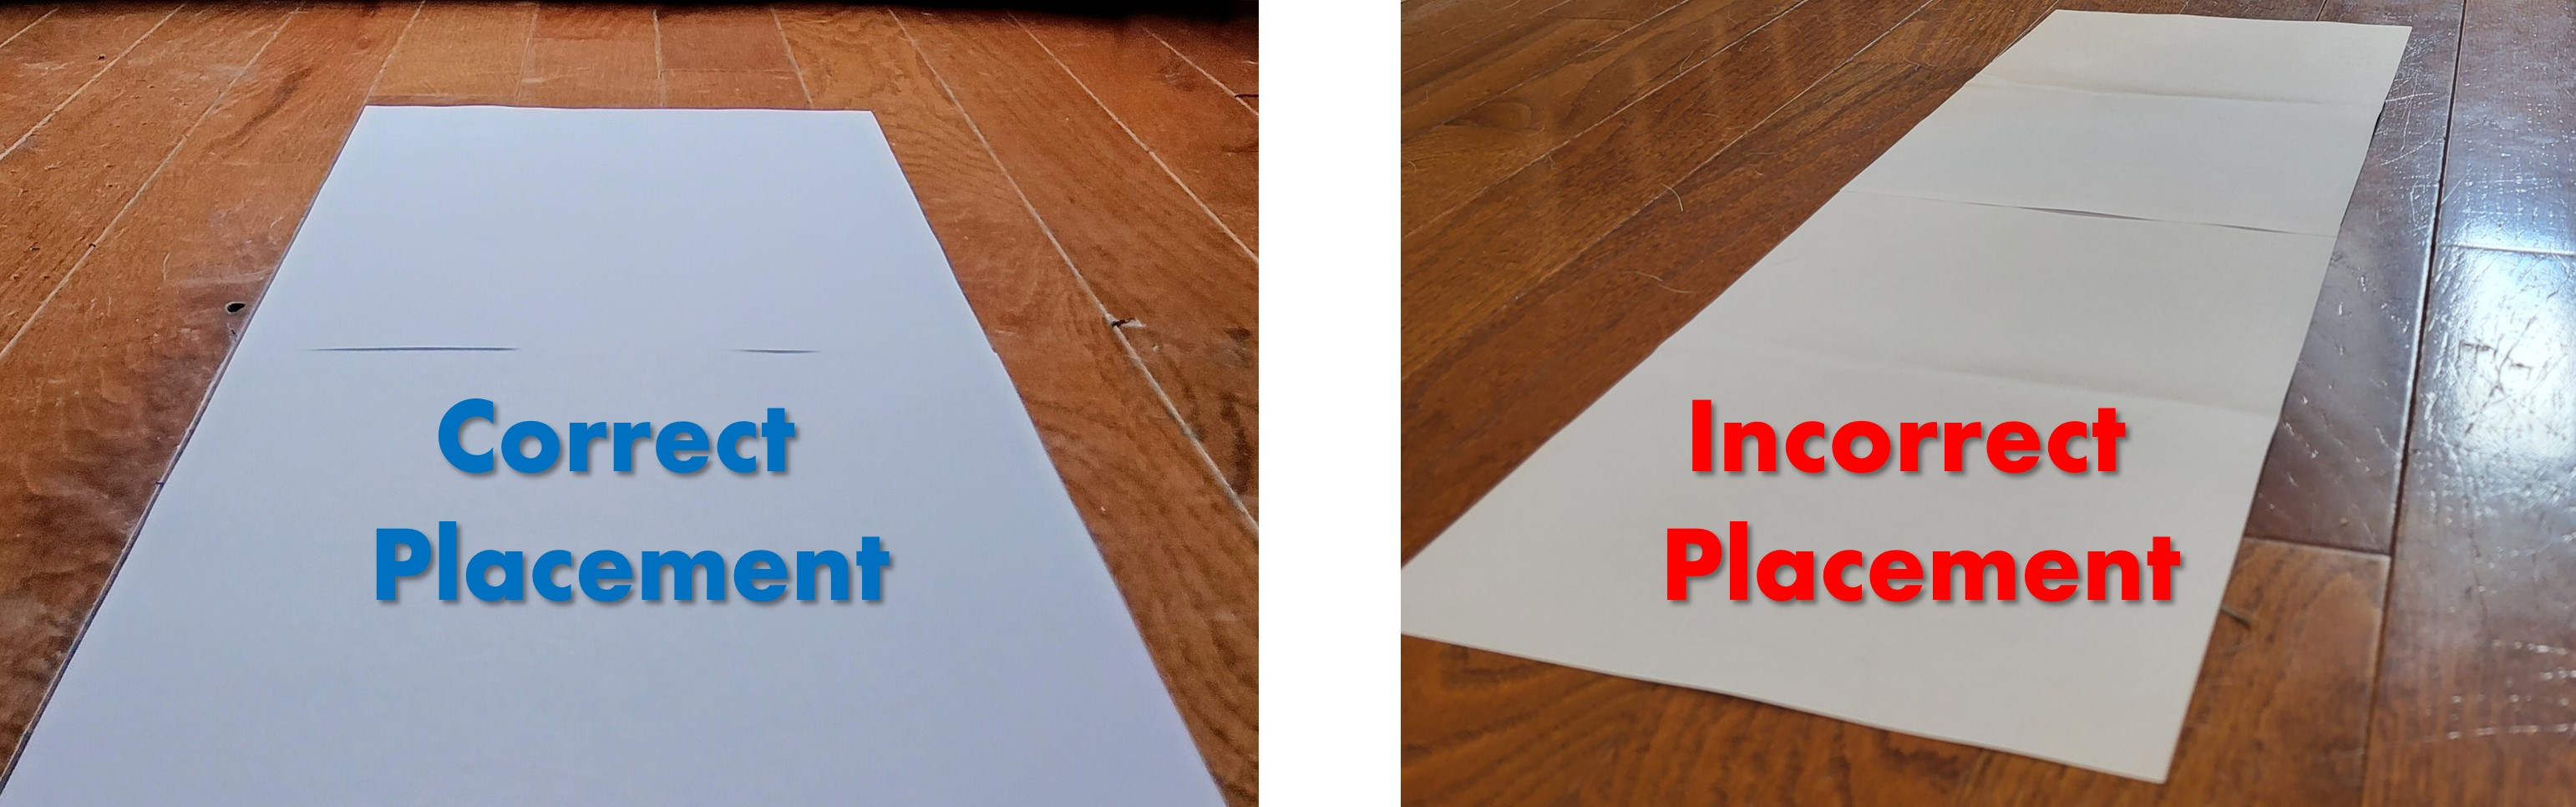
\includegraphics[width=5in]{paperPlacement.jpg}
\end{image}
\item To keep track of the camera height, hold or tape the phone to a meter stick or a ruler. Have one group member record the vertical distance from the surface (hallway floor/desktop/paper) to the camera lens for every shot.  Remember to measure the distance to the camera lens (not the bottom or the top of the phone).
\item Below are two methods for drawing and measuring the triangle.
\begin{enumerate}
    \item \textbf{Method 1.} If you have a touch-screen computer, import your photos into PowerPoint (left) or OneNote (right).  Use the ruler tool (under ''Draw") to outline the edges of the hallway/desk/paper in each photo. Form a triangle with the vanishing point as the top vertex, as shown below.

    \begin{image}
         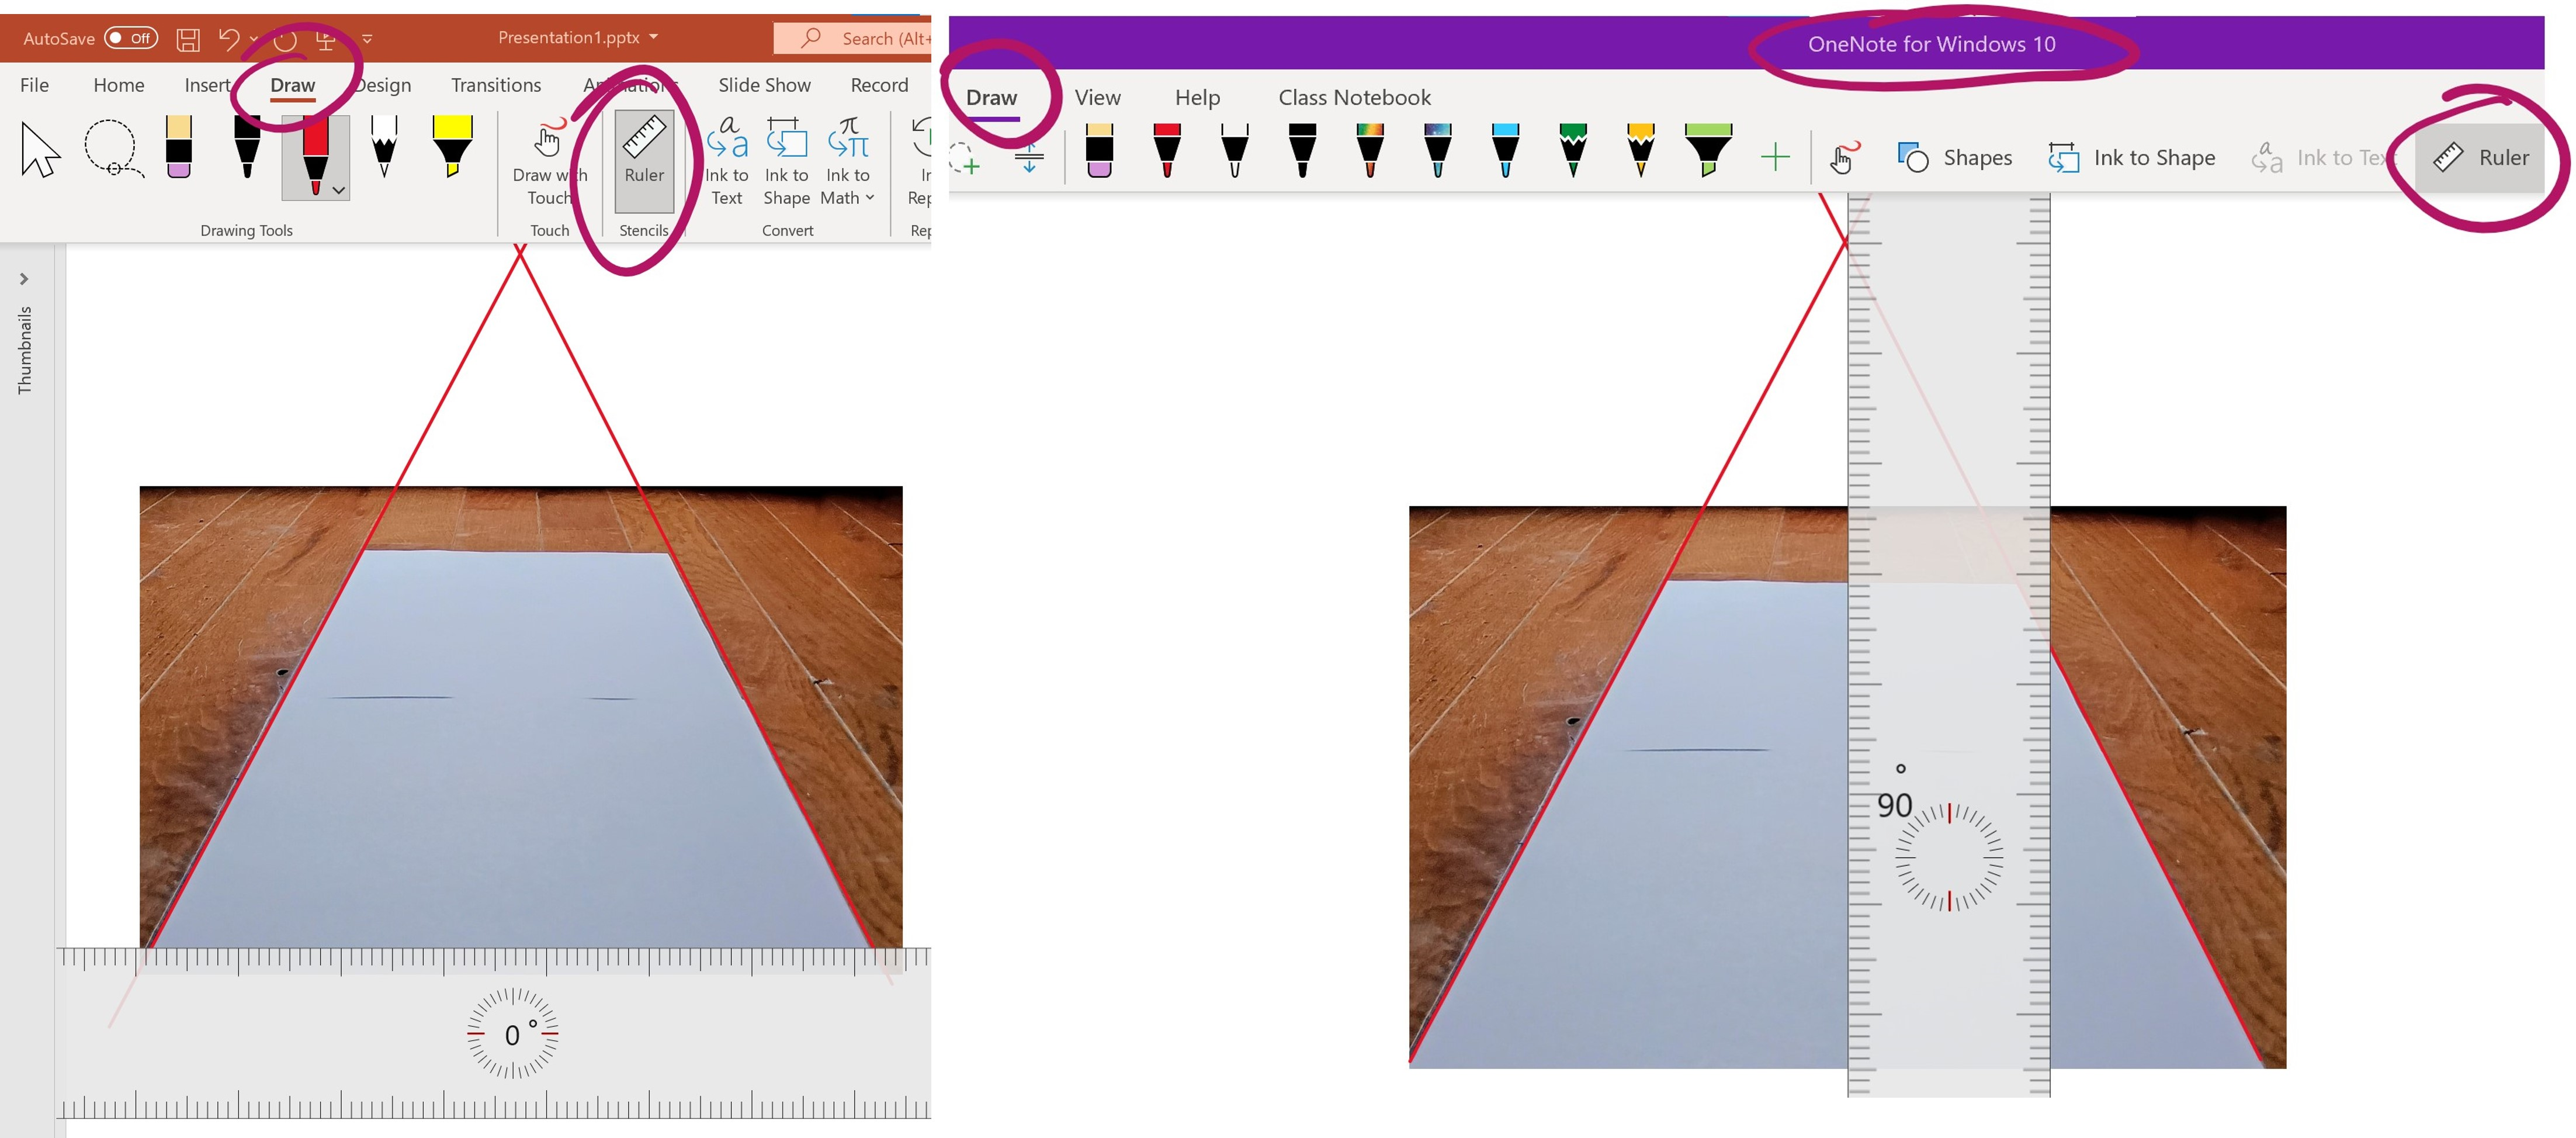
\includegraphics[width=5in]{rulerUse.jpg}
\end{image}

Measure the length of the base, and the height of the triangle and record your measurements.
\item \textbf{Method 2.} You can draw the triangle directly on your phone photo by overlaying a piece of Plexiglass over your photo and using a dry-erase marker and a ruler to trace and extend the edges of the hallway/desk/paper to form a triangle, as shown below (left).

\begin{image}
         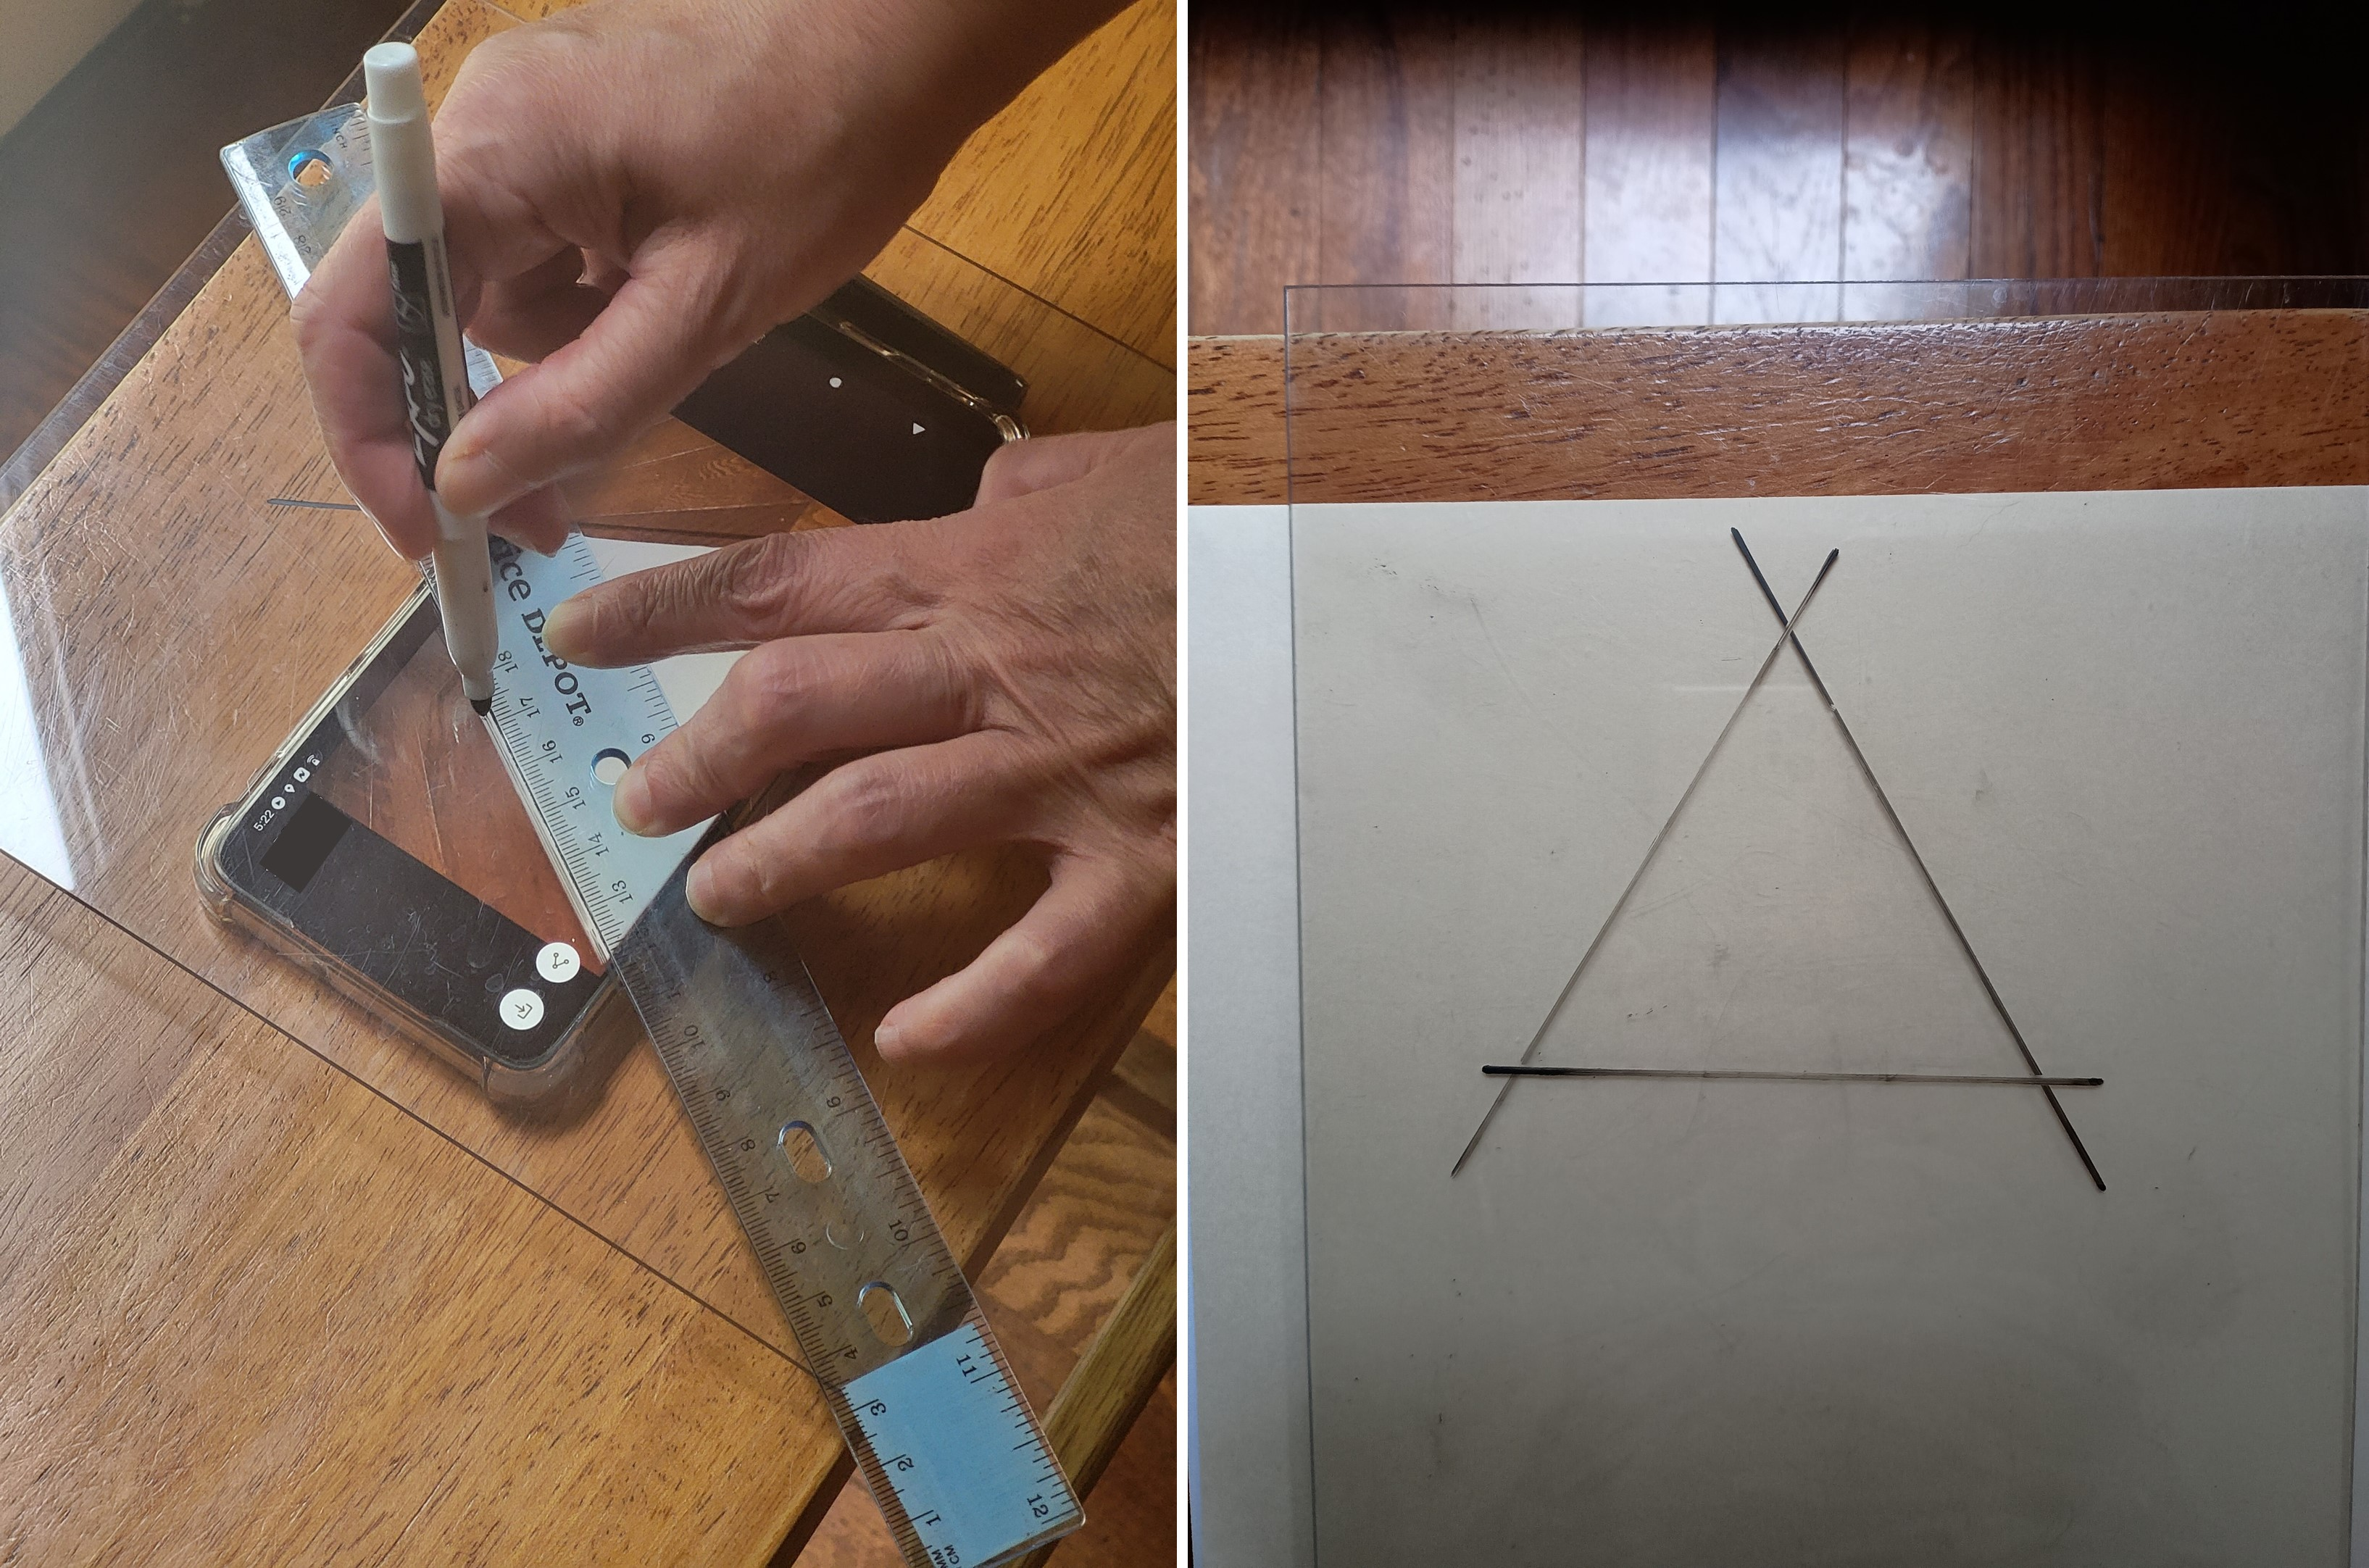
\includegraphics[width=5in]{plexiglass.jpg}
\end{image}

You can now do your measurements on the tracing (right).
\end{enumerate}
\item Follow the procedure you developed in Part 1 to find the height of the camera using ratios.  Compare your computed height to your measured height.  How close did you get?
\end{itemize}

\begin{remark}
    If done carefully, these photo experiments typically produce good results.  If your relative error, $\left(\frac{|\text{measured height}-\text{computed height}|}{\text{measured height}}\right)$, is greater than five percent, consider the following sources of error:
    \begin{itemize}
        \item Did you set up your ratios correctly?  Did you solve the equation correctly?
        \item Is your triangle nearly isosceles?
        \item Did you measure the vertical distance to the actual camera lens? (It is a common mistake to measure the distance to the bottom or the top of the phone.)
        \item When measuring the vertical distance, was the ruler perpendicular to the surface (floor/desktop/paper)? (It is a common mistake to tilt the ruler while measuring.)
    \end{itemize}
\end{remark}

How many examples does it take to prove that our method works in general?  While our examples may be convincing, even a large number of examples is not sufficient to prove that this method works.  What we need to do is develop a theoretical foundation for our method.  This is what we will do in the next part of the activity.

\end{document}